\documentclass{article}
\usepackage{indentfirst}
\usepackage{lmodern}
\usepackage[utf8]{inputenc}
\usepackage[T1]{fontenc}
\usepackage[ngerman]{babel}
\usepackage{amssymb,amstext,amsmath}
\usepackage{graphicx}
\usepackage{dsfont}
\usepackage{amsfonts}
\usepackage{graphics}
\usepackage{float}
\usepackage{cite}
\usepackage{url}
\usepackage{tabularx}
\usepackage{capt-of}
\usepackage{multirow}


\title{Isentropenindex}
\author{Alexander Heinisch, Dominik Wille}
\begin{document}
\maketitle

\vspace{13cm}
\noindent
\begin{center}
\begin{tabular}{r l}
Tutor & Florian Brünig\\
Durchführung & 12. Juni 2013 von 14-18 Uhr \\

E-Mail Dominik & dominik.wille@fu-berlin.de \\
E-Mail Alexander & Matthias.Heinisch@gmx.de \\
\end{tabular}
\end{center}

\newpage
\tableofcontents
\newpage

\section{Ziele des Versuchs}
In diesem experimentell einfachen Versuch sollen wir einen Einblick in die theoretischen Grundlagen der Thermodynamik und der kinetischen Gastheorie bekommen, damit wir Rückschlüsse auf die molekulare Struktur der untersuchten Gase ziehen können.

\section{Physikalische Grundlagen}

\subsection{Die spezifische und die molekulare Wärmekapazität}
Bei der Wärmekapazität unterscheidet man, je nach Zustandsänderung, Hauptsächlich zwischen zwei Arten: \\
{\sc Isochore Zustandsänderung} (konstantes Volumen) \\
Für die Molare Wärmekapazität gilt
\begin{equation}
c_{mv}=\frac{f}{2} \cdot R
\end{equation}
und für die Spezifische Wärmekapazität gilt
\begin{equation}
c_{v}= \frac{f}{2} \cdot \frac{R}{M}
\end{equation}
und {\sc Isobare Zustandsänderung}: (konstanter Druck)\\
Hier gilt für die Molare Wärmekapazität
\begin{equation}
c_{mv}= \left(1+ \frac{f}{2} \right) \cdot R
\end{equation}
und für die Spezifische Wärmekapazität wiederum
\begin{equation}
c_{v}= \left(1+ \frac{f}{2} \right) \cdot \frac{R}{M}
\end{equation}\\

{\begin{center}
\begin{minipage}{\linewidth}
\centering
\makebox[0cm]{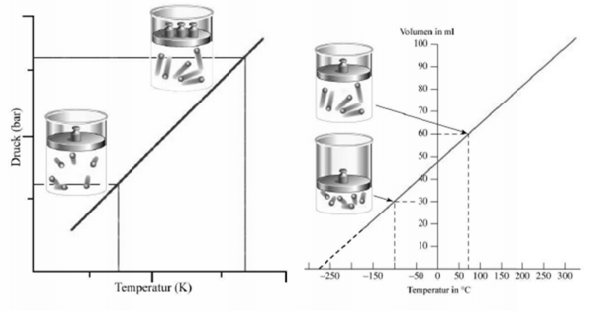
\includegraphics[width=7cm]{Bilder/ise3}}
\captionof{figure}{Schemata der isochoren (links) und isobaren Zustandsänderung (rechts)}
\label{sch}
\end{minipage}
\end{center}

\subsection{Die Poisson-Gleichung}
Sobald ein Prozess ohne den Austausch von Energien, ohne adiabatische oder reversieble Zustandsänderung und ohne Energieerzeugung stattfindet, nennt man ihn isotrop. Aus dem ersten Hauptsatz der Thermodynamik lassen sich die Poisson-Gleichungen ableiten, welche isotrope Prozesse von idealen Gasen beschreiben.\\

Dabei gilt für adiabatische Prozesse \((dQ=0)\):

\begin{equation}
\label{1}
dU=dQ-p \cdot dV
\end{equation}

Die Innere Energie wird wie folgt definiert:

\begin{equation}
\label{2}
dU=c_{v} \cdot dT
\end{equation}

Und damit:

\begin{equation}
\label{3}
dU=c_{v} \cdot dT=-p \cdot dV
\end{equation}

p ist die allgemeine Gasgleichung 

\begin{equation}
\label{4}
p= \frac{R \cdot T}{V}
\end{equation}

Das alles nun in Gl.\(\eqref{3}\) zusammengeführt ergibt:

\begin{equation}
\label{5}
c_{v} \cdot dT=- \frac{R \cdot T}{V} \cdot dV
\end{equation}

Beziehungsweise mit Trennung der Variablen: 

\begin{equation}
c_{v}\cdot\frac{dT}{T}=-R\cdot\frac{dV}{V}
\end{equation}

Nun Integrieren wir beide Seiten und erhalten:

\begin{equation}
c_{v}\cdot ln(T)=-R\cdot ln(V)+const
\end{equation}

Beziehungsweise:

\begin{equation}
ln(T^{c_{v}} +V^R )=const
\end{equation}

Nun ersetzten wir die allgemeine Gaskonstante R mit \(R=c_{p}-c_{v}\)
woraus folgt:

\begin{equation}
T^{c_{v}}\cdot V^{(c_{p}-c_{v})}=const
\end{equation}

mit der \(c_{v}\)-ten Wurzel haben wir nun:

\begin{equation}
T\cdot V^{(\kappa -1)}=const
\end{equation}

\(\kappa\) ist der adiabaten Koeffizient auf den wir später noch eingehen werden:

\begin{equation}
\kappa =\frac{c_{p}}{c_{v}}
\end{equation}

Gl.\(\eqref{4}\) nach T umgestellt und eingesetzt ergibt schließlich die Poisson-Gleichung:

\begin{equation}
\label{16}
p\cdot V^\kappa =const
\end{equation}

\subsection{Der Isotropenindex}
\(\kappa\) beschreibt das Verhältnis der spezifischen Wärmekapazitäten für den Fall, dass der Druck und das Volumen konstant bleiben:

\begin{equation}
\kappa =\frac{c_{p}}{c_{v}}=\frac{c_{mp}}{c_{mv}}
\end{equation} 

Daraus folgt in Abhängigkeit von den Molekülen:

\begin{equation}
\label{18}
\kappa =\frac{c_{p}}{c_{v}}=\frac{\left(1+\frac{f}{2}\right)\cdot \frac{R}{M}}{\frac{f}{2}\cdot \frac{R}{M}}=\frac{f+2}{f}=1+\frac{2}{f}
\end{equation}

\subsection{Die Methode nach Clement-Desormes}
Clement-Desormes hatte die Idee, die schwierige Messung einer kleinen Temperaturänderung eines Gases auf eine einfache Druckmessung zurückzuführen. Somit lässt sich \(\kappa\) dieses Gases bestimmen.  
Dabei wird das Gas mit einem bekannten Volumen V in einen geeigneten Behälter eingeschlossen. Bei kurzzeitigen Zustandsänderungen kann der Wärmeaustausch mit dem Gehäuse vernachlässigt werden. Die Differenz zwischen dem Gasdruck \(p\) und dem äußeren Druck \(p_{a}\) messen wir über einen offenen Manometer, dabei ist die Höhendifferenz \(\Delta\)h proportional zur Druckdifferenz. Wir untersuchen dabei eine adiabatische Zustandsänderung (a) von \((p_{1} T_{1} = T_{A})\) mit \(p_{1} > p_{A}\) und \(T_{A}\) = Raumtemperatur auf \((p_{2} = p_{A}, T_{2})\) und anschließend eine isochore (V=const) Zustandsänderung (i) auf \(\ (p_{3}, T_{3}=T_{A})\)(siehe Skizze).\\

\begin{center}
\begin{minipage}{\linewidth}
\centering
\makebox[0cm]{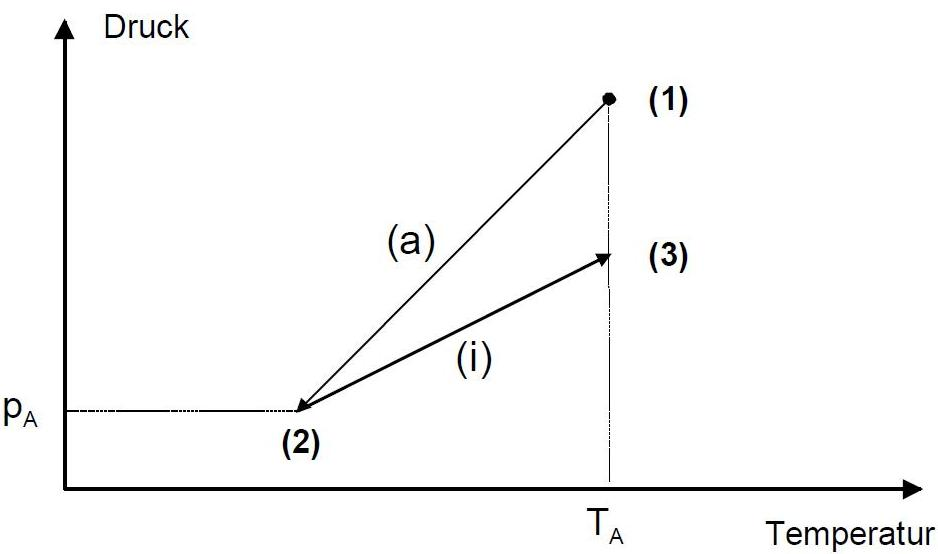
\includegraphics[scale=0.3]{Bilder/ISE.jpg}}
\captionof{figure}{adibate Zustandsänderung (Quelle: GP I Skript, Freie Universität Berlin)}
\label{wtd}
\end{minipage}
\end{center}

Bei der Durchführung des Versuchs wird Anfangs ein leichter Überdruck in dem Gefäß erzeugt. Anschließend wartet man, bis der Temperaturausgleich vollzogen ist \(T_{1}=T_{A}\). Anschließend öffnen wir ein Ventil, was zum einen zur Folge hat, dass sich das Gas adiabatisch entspannt bis es sich an den Außendruck angepasst hat \((p_{2} = p_{A})\), und zum anderen verringert sich seine innere Energie und Temperatur (siehe Versuchsaufbau Abbildung 3). Die Temperaturabnahme kann man mithilfe der {\sc Poisson-Gleichung} berechnen. Als Nächstes erwärmt sich das Gas wieder isochor auf \(T_{3}\) auf, bis es den Punkt \(p_{3}\) erreicht. Dieser Druckanstieg lässt sich durch die allgemeine Zustandsgleichung berechnen. Da die Druck- und Temperaturänderungen relativ klein sind, betrachten wir die Näherung \(dp\approx \Delta p\) differentiell. Daraus folgt für die {\sc Poisson-Gleichung}:

\begin{equation}
p^{1-\kappa }\cdot T^\kappa =const
\end{equation}

Das totale Differential und eine Umformung liefert uns:

\begin{equation}
\label{10}
(1-\kappa )\frac{dp_{a}}{p}+\kappa \frac{dT_{a}}{T}=0
\end{equation}

Für die isochore Zustandsänderung gilt:
\begin{equation}
\label{11}
\frac{p}{T}=const \notag
\end{equation}
\begin{equation}
\frac{dp_{i}}{T}-p \frac{dT_{i}}{T^2}=0 \hspace{1cm} bzw. \hspace{1cm} \frac{dT_{i}}{T}=\frac{dp_{i}}{p}
\end{equation}

Wenn wir jetzt Gl.\(\eqref{10}\) mit \(dT_{i}=-dT_{a}\) in Gl.\(\eqref{11}\) einsetzten, ergibt sich:

\begin{equation}
(1-\kappa ) \frac{dp_{a}}{p}-\kappa \frac{dp-{i}}{p}=0 \notag
\end{equation}

\begin{equation}
\label{kappa}
\kappa =\frac{dp_{a}}{dp_{a}+dp_{i}}\approx \frac{\Delta h_{1}}{\Delta h_{1}-\Delta h_{3}}
\end{equation}

Dabei ist \(h_{1}\) und \(h_{3}\) die Höhendifferenz am Manometer am Anfangszustand 1 und Endzustand 3. Gl.\(\eqref{kappa}\) ist die Messvorschrift der Messmethode von Clement-Desormes. Ein Nachteil ist allerdings, dass aufgrund der niedrigen Druckdifferenz bzw. des kleinen Höhenunterschieds die Messgenauigkeit nicht sehr hoch ist.

\begin{center}
\begin{minipage}{\linewidth}
\centering
\makebox[0cm]{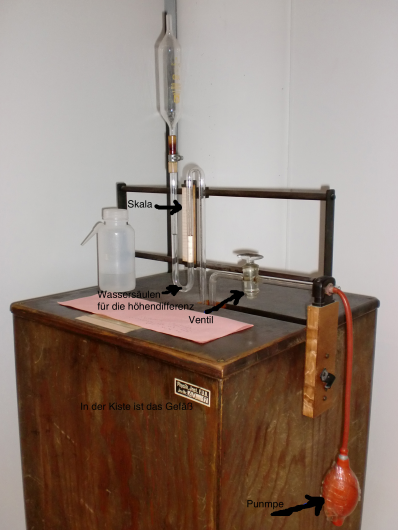
\includegraphics[width=7cm]{Bilder/ise1}}
\captionof{figure}{Aufbau zum Clement-Desormes Verfahren aus dem GP-Gebäude}
\label{wtd}
\end{minipage}
\end{center}

\subsection{Die Methode nach Flammersfeld-Rüchert}
Im Gegensatz zu Clement-Desormes Methode hat Rücherts Schwingungsmethode den Vorteil der höheren Messgenauigkeit. Es wird ein Gasvolumen durch einen beweglichen Kolben abgeschlossen welcher in einem Präzisionsglasrohr schwingt (siehe Abbildung 4). Das Volumen und der Druck bestimmen dabei die Rückstellkraft und damit die Eigenfrequenz des Kolbens. Diese können wir mithilfe der Adiabatengleichung berechnen. Der Nachteil dieser Methode war die geringe Anzahl der Perioden, wodurch die Messung ebenfalls an Genauigkeit verliert. Flammersfeld verbesserte den Aufbau, indem er durch eine parametrische Selbststeuerung eine stationäre Schwingung erreichte. Er gleichte den Gas- und Energieverlust durch eine kleine Öffnung an der Mittellage des Kolbens aus, durch welchen eine kleine Gasströmung entstand.
Befand sich nun der Kolben unterhalb der Öffnung, verzerrte sich die Schwingung durch die Erhöhung des Gasdrucks. War der Kolben oberhalb des Lochs, ließ sich seine Bewegung durch einen freien Fall mit starker Reibung beschreiben. Entgegen der Erwartungen, war die Störung durch die Reibung sehr viel kleiner und die Eigenfrequenz wurde nur schwach beeinflusst.
\newpage
Nun bilden wir von Gl.\(\eqref{16}\) das totale Differential und erhalten:

\begin{equation}
\frac{dp}{p}+\kappa \frac{dV}{V}=0
\end{equation}

wobei p der Druck ist und V das Volumen. Für die Rückstellkonstante D gilt:

\begin{equation}
D=-\frac{dF}{dx}=-\frac{Sdp}{dx}=\kappa \frac{pS^2}{V}
\end{equation}

Hier entspricht dx und dF der Auslenkung und der Kraft auf den Kolben bzgl. der Ruhelage und S ist die Querschnittsfläche. Als Eigenfrequenz erhalten wir nun:

\begin{equation}
\label{25}
\omega_{0}^2=\frac{D}{m}=\kappa \frac{pS^2}{mV} \hspace{1cm} und \hspace{1cm} \kappa =\frac{4\pi ^2}{\tau ^2} \frac{mV}{pS^2}
\end{equation}

Hierbei sind nun m die Masse und \(\ \tau\) die beobachtete Periodendauer.

{\begin{center}
\begin{minipage}{\linewidth}
\centering
\makebox[0cm]{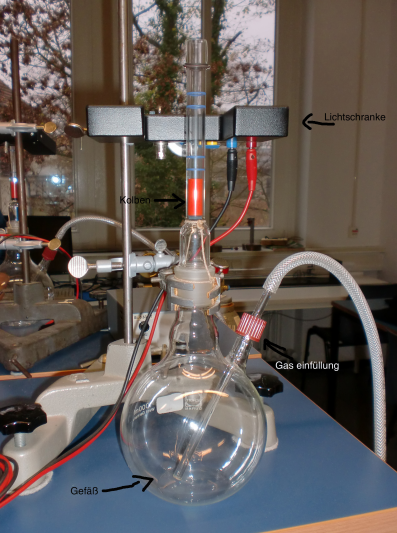
\includegraphics[width=7cm]{Bilder/ise2}}
\captionof{figure}{Aufbau zum Flammersfeld-Rüchert Verfahren aus dem GP-Gebäude}
\label{wtd}
\end{minipage}
\end{center}

\newpage
\subsection{Freiheitsgrade}
Die Anzahl der Freiheitsgrade eines Gases bestimmt die Zahl der wählbaren, voneinander unabhängigen Bewegungsmöglichkeiten eines Systems. In der Thermodynamik verteilt sich Energie, welche man einem Gas hinzu führt, stets gleichmäßig auf die einzelnen Freiheitsgrade. Beschrieben wird diese Verteilung durch die Entropie. Da ein Gas aus vielen einzelnen Atomen besteht und es unmöglich ist, die \(10^{23}\) Freiheitsgrade zu bestimmen, hat man den Begriff des Idealen Gases eingeführt. Man betrachtet das Gas in einem Volumen V unter der Annahme, dass nur eine Art von Atomen sich in diesem Volumen befinden (Ideales Gas). So reduziert man die \(10^{23}\) Freiheitsgrade auf die, des einzelnen Atoms:

\vspace{1cm}
\begin{tabular}{l|l|l|l|l}
Gasmolekül & \multicolumn{4}{c}{Anzahl der Freiheitsgrade}\\
\hline
& Translation & Rotation & Schwingung (doppelt zu zählen) & Summe\\
\hline
1-atomig & 3 & 0 & 2x(3x1-3-0)=0 & 3\\
2-atomig & 3 & 2 & 2x(3x2-3-2)=2 & 7\\
3-atomig linear & 3 & 2 & 2x(3x3-3-2)=8 & 13\\
3-atomig gewinkelt & 3 & 3 & 2x(3x3-3-3)=6 & 12\\ 
\end{tabular}

\vspace{2cm}
\section{Aufgaben}
\subsection{Aufgabe 1}
Bestimmung des Verhältnisses der spezifischen Wärmen \(\ \frac{c_{p}}{c_{v}}=\kappa \) für Luft nach der Methode von {\sc Clement-Desormes}.
\subsection{Aufgabe 2}
Bestimmung des Wertes für \(\ \kappa \)  für ein einatomiges (Argon), ein zweiatomiges \(\ (N_{2}\)) und ein dreiatomiges Gas \(\ (CO_{2})\) durch Messung der Eigenfrequenzen des Gasoszillators.\\
Vergleich der Ergebnisse untereinander und mit den erwarteten Werten aus der kinetischen Gastheorie für ein ideales Gas.

\newpage

\section{Beobachtung und Auswertung}
\subsection{Aufgabe 1 - Die Methode des Clement-Desormes}
\subsubsection{Beobachtung}
Um diese Aufgabe zu lösen, benutzten wir die Apparatur von Clement-Desormes, deren Aufbau schon in der Vorbereitung erklärt wurde. Wir pumpten so viel Luft in das Röhrchen, bis die linke Wassersäule einen Wert von 100-110cm und die rechte Säule einen Wert von 20-30cm erreicht hatten. Anschließend schlossen wir das Ventil und warteten etwa eine Minute, bis sich ein Gleichgewicht eingestellt hatte. Danach öffneten wir das Ventil kurz, damit beide Wassersäulen wieder in ihr mittleres Gleichgewicht zurück fielen bzw. stiegen. Nach dem erneuten Schließen des Ventils warteten wir vier Minuten. In dieser Zeit stieg die rechte, bzw. fiel die linke Säule wieder. Diesen Vorgang wiederholten wir insgesamt drei Mal.\\

\subsubsection{Auswertung}
In der folgenden Tabelle sind unsere Messergebnisse der Höhendifferenzen der Wassersäulen jeweils zu Beginn und am Ende der jeweiligen Messreihe \(\Delta h_1\) und \(\Delta h_2\) festgehalten. Der Fehler entspricht dem geschätzten Ablesefehler:
\\

\vspace{1cm}
\begin{center}
\begin{tabular}{c|c}
\(\Delta h_1\) [mm] & \(\Delta h_2\)[mm]\\
\hline
\(102 \pm 1\) & \(27\pm 1\)\\
\(86 \pm 1\) & \(33\pm 1\)\\
\(91 \pm 1\) & \(24\pm 1\)\\
\end{tabular}
\end{center}
\captionof{table}{Messwerte der Höhendifferenzen}

\vspace{1cm}
Gemittelt ergibt sich für \(\overline{\Delta h_1}\) und für \(\overline{\Delta h_2}\).
\begin{center}
\(\overline{\Delta h_1} = (93\pm 4.73)\)mm\\
\(\overline{\Delta h_2} = (28\pm 2.65)\)mm
\end{center}

Der Fehler errechnet sich aus der Standartabweichung:
\begin{equation}
\notag
\Delta (\overline{\Delta h_i}) = \sqrt{\frac{1}{n}\frac{1}{n-1}\sum\limits_{i}(h_i \ - \overline{h})^2}
\end{equation}
\newpage
Um jetzt aber \(\kappa\) zu bestimmen, benutzen wir Gl.\(\eqref{kappa}\) und erhalten einen Wert von:

\begin{center}
\(\kappa = (1.43\pm 0.15)\)
\end{center}

\(\Delta\kappa\) errechnet sich aus der Gauß'schen Fehlerfortpflanzung:
\begin{equation}
\notag
\Delta\kappa = \sqrt{\left({\frac{\Delta \left(\Delta h_1\right)}{\Delta h_1}}\right)^2+\left(\frac{\Delta (\Delta h_2)}{\Delta h_2}\right)^2} \cdot\kappa
\end{equation}

Der theoretische Wert für den Isentropenindex der Luft errechnen wir aus Gl.\(\eqref{18}\). Dabei beachten wir, dass Luft ein Gemisch aus vielen verschiedenen Gasen ist. Der Hauptanteil liegt allerdings mit \(87\%\) bei Stickstoff und mit \(21\%\) bei Sauerstoff. Alle anderen Anteile sind zu klein und können vernachlässigt werden. Beide Gase bestehen aus zweiatomige Molekülen, woraus folgt, dass wir 5 Freiheitsgrade haben. Daraus ergibt sich für \(\kappa_{theo}\):

\begin{equation}
\notag
\kappa_{theo} = \frac{2+f}{f} = 1.4
\end{equation}
 
Was mit unserem experimentell bestimmten Wert identisch ist.

\subsubsection{Fazit}
Der Versuch verlief reibungslos und wir hatten keine Probleme mit der Apparatur. Dass das Ergebnis für \(\kappa\) mit den theoretischen Erwartungen identisch ist, liegt wahrscheinlich daran, dass wir uns viel Zeit genommen haben und gewartet hatten, bis die Wassersäulen sich gar nicht mehr bewegt haben.

\vspace{1 cm}
\subsection{Aufgabe 2 - Die Methode des Flammersfeld-Rüchert}
\subsubsection{Auswertung}
Für diese Aufgabe ließen wir die verschiedenen Gase Argon, Stickstoff und Kohlenstoffdioxid in die Apparatur von Flammersfeld-Rüchert strömen. Mit Handstoppuhren haben wir die Zeit gemessen und eine Lichtschranke zählte die Anzahl der Kolbenbewegungen. In der folgenden Tabelle werden die aus dem Skript entnommenen Informationen über das Arbeitsvolumen der Gase, die Kolbenmasse, sowie der Durchmesser des Kolbens aufgelistet.

\begin{center}
\begin{tabular}{l|c|c|c|l}
& {$N_2$} & {$CO_2$}& {$Ar$}& {Fehler}\\
\hline 
Arbeitsvolumen/\(cm^3\)  & 1145 & 1147 & 1142 & \(\pm\) 3,00 \\ 
Kolbenmasse/g  & 4,58 & 4,50 & 4,52 & \(\pm\) 1,00\\ 
Kolbendurchmesser/mm & 11,90 & 11,90 & 11,90 & \(\pm\) 0,03\\
\end{tabular}
\end{center}
\captionof{table}{Daten zu den verwendeten Gasen und Kolben}

\newpage
In dem Raum Herrschte während unserer Versuche ein Druck von\\ p=(\(1012\pm 3)\) mbar

\subsubsection{Bestimmung des Isentropenindex von Argon}
Zuerst bestimmen wir die Periodendauer \(\tau_{1}\) der Schwingungen. Wir ließen den Kolben beim ersten Durchlauf 300 Mal, und bei den darauffolgenden 9 nur noch 100 Schwingungen 
durchführen. Dabei erhielten wir für Argon folgende Messwerte:

\begin{center}
\begin{tabular}{c|c|c}
Schwingungen & gemessene Zeit [s]& Zeit/Schwingung [t]\\
\hline 
\(300\)	& \(108,16\)& \(0,3610\)\\
\(100\)	& \(32,42\)	& \(0,3242\)\\
\(100\)	& \(32,52\)	& \(0,3252\)\\
\(100\)	& \(32,51\)	& \(0,3251\)\\
\(100\)	& \(32,66\)	& \(0,3266\)\\
\(100\)	& \(32,45\)	& \(0,3245\)\\
\(100\)	& \(32,57\)	& \(0,3257\)\\
\(100\)	& \(32,72\)	& \(0,3272\)\\
\(100\)	& \(32,73\)	& \(0,3273\)\\
\(100\)	& \(32,65\)	& \(0,3265\)\\
\end{tabular}
\end{center}
\captionof{table}{Rohwerte für Argon}

\vspace{1cm}

Als Mittelwert für die Periodendauer ergibt sich ein Wert von:
\begin{center}
\(\overline{\tau}_{1} = (0.3293 \pm 0.0035)\)s
\end{center}

Der Fehler von \(\overline{\tau}_{1}\) errechnen wir wieder über die Standartabweichung:

\begin{equation}
\Delta \overline{\tau}_{1} = \sqrt{\frac{1}{n} \frac{1}{n-1}\sum\limits_{i}(x_i \ - <x>)^2}
\end{equation}

Unter Verwendung von Gl.\(\eqref{25}\) erhalten wir für \(\kappa_{Argon}\) den Wert:
\begin{center}
\(\kappa_{Argon} = (1.29 \pm 0.05)\)
\end{center}
Der Fehler errechnet sich wieder über die Gauß'sche Fehlerfortpflanzung:
\begin{equation}
\notag
\Delta \kappa_1 =\sqrt{\left( \frac{ -2mV}{ \tau^3 p r^4}\cdot \Delta \tau\right)^2 + \left( \frac{ 4V}{\tau^3 p r^4}\cdot \Delta m \right)^2+\left( \frac{4m }{\tau^3 p r^4}\cdot\Delta V \right)^2+\left( \frac{-4mV}{\tau^3 p^2 r^4}\Delta p \right)^2+\left( \frac{-16mV}{\tau^3 p r^5}\Delta r \right)^2}
\end{equation}

Der theoretische Wert für Argon liefert uns wieder Gl.\(\eqref{kappa}\) wobei Argon 3 Freiheitsgrade hat:
\begin{equation}
\notag
\kappa_{theo} = \frac{2+f}{f} = 1.67
\end{equation}

\subsubsection{Bestimmung des Isentropenindex von Kohlenstoff}
Wir gingen exakt wie bei Argon vor und erhielten folgende Messwerte:
\begin{center}
\begin{tabular}{c|c|c}
Schwingungen & gemessene Zeit [s]& Zeit/Schwingung [t]\\
\hline 
\(300\)	& \(108,63\) & \(0,3621\)\\
\(100\)	& \(36,06\)	& \(0,3606\)\\
\(100\)	& \(35,97\)	& \(0,3597\)\\
\(100\)	& \(35,82\)	& \(0,3582\)\\
\(100\)	& \(35,91\)	& \(0,3591\)\\
\(100\)	& \(35,87\)	& \(0,3587\)\\
\(100\)	& \(35,85\)	& \(0,3585\)\\
\(100\)	& \(36,06\)	& \(0,3606\)\\
\(100\)	& \(35,78\)	& \(0,3578\)\\
\(100\)	& \(35,87\)	& \(0,3587\)\\
\end{tabular}
\end{center}
\captionof{table}{Rohwerte für Kohlenstoff}

\vspace{1cm}

Als Mittelwert für die Periodendauer ergibt sich ein Wert von:
\begin{center}
\(\overline{\tau}_{2} = (0.3594 \pm 0.0005)\)s
\end{center}

Der Fehler errechnet sich wieder schon zuvor über die Gauß'sche Fehlerfortpflanzung.
Wir verwenden wieder Gl.\(\eqref{25}\) und erhalten für die Periodendauer:
\begin{center}
\(\kappa_{CO_2} = (1.07 \pm 0.05)\)
\end{center}

Der theoretische Wert für CO\(_2\) liefert uns wieder Gl.\(\eqref{kappa}\) wobei CO\(_2\) 9 Freiheitsgrade hat:
\begin{equation}
\notag
\kappa_{theo} = \frac{2+f}{f} = 1.23
\end{equation}

\subsubsection{Bestimmung des Isentropenindex von Stickstoff}
Zuletzt berechnen wir noch den Isentropenindex von Stickstoff. Auch hier sind wir wie in den zwei Versuchen vorher schon, genau gleich vorgegangen.
\newpage
\begin{center}
\begin{tabular}{c|c|c}
Schwingungen & gemessene Zeit [s]& Zeit/Schwingung [t]\\
\hline 
\(100\)	& \(35,66\)	& \(0,3566\)\\
\(100\)	& \(35,43\)	& \(0,3543\)\\
\(100\)	& \(35,46\)	& \(0,3546\)\\
\(100\)	& \(35,23\)	& \(0,3523\)\\
\(100\)	& \(35,49\)	& \(0,3549\)\\
\(100\)	& \(35,33\)	& \(0,3533\)\\
\(100\)	& \(35,27\)	& \(0,3527\)\\
\(100\)	& \(35,01\)	& \(0,3501\)\\
\(100\)	& \(35,70\)	& \(0,3570\)\\
\(100\)	& \(35,43\)	& \(0,3543\)\\
\end{tabular}
\end{center}
\captionof{table}{Rohwerte für Stickstoff}

\vspace{1cm}
Als Mittelwert für die Periodendauer ergibt sich ein Wert von:
\begin{center}
\(\overline{\tau}_{3} = (0.3540 \pm 0.0006)\)s
\end{center}

Der Fehler errechnet sich auch hier wieder wie schon zuvor, über die Gauß'sche Fehlerfortpflanzung.
Wir verwenden wieder Gl.\(\eqref{25}\) und erhalten für die Periodendauer:
\begin{center}
\(\kappa_{N_2} = (1.13 \pm 0.05)\)
\end{center}

Der theoretische Wert für N\(_2\) liefert uns erneut Gl.\(\eqref{kappa}\) wobei N\(_2\) 5 Freiheitsgrade hat:
\begin{equation}
\notag
\kappa_{theo} = \frac{2+f}{f} = 1.40
\end{equation}

\subsubsection{Fazit}
Unsere Ergebnisse für die Isotropenindizes sind bei jedem Gas kleiner als die theoretisch erwarteten Werte. Das legt einen möglichen systematischen Fehler nahe. Die verwendeten Formeln setzen die Benutzung eines idealen Gases voraus, was nur sehr schwer herstellbar ist, womit wir eine mögliche Fehlerquelle haben. Des weiteren könnte es auch am Luftdruck, welcher am Versuchstag gemessen wurde, liegen, oder die Kolben liefen nicht so gleichförmig wie angenommen.

\newpage
\section{Zusammenfassung}
In Aufgabe 1 haben wir die Methode von Clement-Desormes benutzt, um den Isentropenindex von normaler Luft zu bestimmen. Bei diesem Versuch haben wir dem verwendeten Gas viel Zeit gegeben um sich, nach dem das Ventil kurz geöffnet wurde, wieder auszudehnen. Das erhaltene Ergebnis von \(\kappa = (1.43 \pm 0.15) \) ist identisch mit dem theoretisch erwarteten Wert \(\kappa_{theo}=1.4\).\\
Bei Aufgabe 2 sollten wir die Periodendauer und die Isentropenindizes für die Gase Argon, Stickstoff und Kohlenstoffdioxid berechnen. Stellen wir nun die experimentelle und theoretische Werte tabellarisch dar:

\begin{center}
\begin{tabular}{l|c|c|c}
& \(\tau\) & \(\kappa_{exp}\) & \(\kappa_{theo}\)\\
\hline
Ar &  \(0.3293\pm 0.0035\) & \(1.29\pm 0.05\) & 1.67\\
N\(_2\) & \(0.3540\pm 0.0006\) & \(1.13\pm 0.05\) & 1.40\\
CO\(_2\) & \(0.3594\pm 0.0005\)  & \(1.07\pm 0.05\) & 1.23\\
\end{tabular}
\end{center}
\captionof{table}{Ergebnisse Aufgabe 2}
\vspace{1cm}
Die Werte für die Periodendauer haben einen so geringen Fehlerwert, weil wir pro Messreihe den Kolben 100 Mal die Oszillation durchführen ließen. Trotzdem liegen alle unsere bestimmten Werte unter den theoretisch Erwarteten. Als Grund dafür müssen wir einen systematischen Fehler annehmen, da die Daten aus dem Skript, welche zur Bestimmung der \(\kappa\) benutzt wurden, alles Konstante sind (Durchmesser/Gewicht des Kolben und Arbeitsvolumen der Gase). Als Möglichkeiten stünde noch zur Verfügung, dass die Kolben nicht so harmonisch Oszilliert haben wie wir vom Augenmaß her annahmen oder dass wir womöglich eben nicht mit idealen Gasen gearbeitet haben.

\section{Quellenangabe}
\begin{itemize}
\item Platzskript
\item Als Orientierung für die Theoretischen Grundlagen wurde das GP2-Skript herangezogen
\item Wikipedia
\end{itemize}
\vspace{3.0cm}

\begin{tabularx}{\textwidth}[b]{p{5cm} X p{5cm}} \cline{1-1} \cline{3-3}
Datum, Dominik Wille & & Datum, Alexander Heinisch
\end{tabularx}
\end{document}